\documentclass[12pt]{article}
\usepackage{bussproofs, array, amstext, amssymb} 
\usepackage{mathtools, extarrows}
\usepackage{latexsym}
\usepackage{syntax}
\usepackage{tabularx}
\usepackage{flowchart}
\usepackage{array,multirow}
\usepackage[section]{placeins}
\usepackage[bottom]{footmisc}
\usepackage{tablefootnote}
% \usepackage[nodayofweek,level]{datetime}
\usepackage[affil-it]{authblk}
\usepackage{hyperref}
\usepackage{algorithm,algpseudocode}
\usepackage{textcomp}
\usepackage{pgfplots}
\usepackage[utf8]{inputenc}
\usepackage[T1]{fontenc}
\usepackage{catchfilebetweentags}
\usepackage{agda}
\usepackage[verbose]{newunicodechar}
\usepackage{bigfoot}
\usepackage{makecell}

\newunicodechar{ᵇ}{\ensuremath{\mathnormal{\sp{b}}}}
\newunicodechar{⊎}{\ensuremath{\mathnormal{\uplus}}}
\newunicodechar{₁}{\ensuremath{\mathnormal{\sb{1}}}}
\newunicodechar{₂}{\ensuremath{\mathnormal{\sb{2}}}}
\newunicodechar{≤}{\ensuremath{\mathnormal{\le}}}
\newunicodechar{≈}{\ensuremath{\mathnormal{\approx}}}
\newunicodechar{∀}{\ensuremath{\mathnormal{\forall}}}
\newunicodechar{∃}{\ensuremath{\mathnormal{{\exists}}}}
\newunicodechar{≡}{\ensuremath{\mathnormal{\equiv}}}
\newunicodechar{Γ}{\ensuremath{\mathnormal{\Gamma}}}
\newunicodechar{λ}{\ensuremath{\mathnormal{\lambda}}}
\newunicodechar{ϕ}{\ensuremath{\mathnormal{\phi}}}
\newunicodechar{ψ}{\ensuremath{\mathnormal{\psi}}}
\newunicodechar{∷}{\ensuremath{\mathnormal{::}}}
\newunicodechar{⊤}{\ensuremath{\mathnormal{\top}}}
\newunicodechar{⊥}{\ensuremath{\mathnormal{\bot}}}
\newunicodechar{∨}{\ensuremath{\mathnormal{\lor}}}
\newunicodechar{∧}{\ensuremath{\mathnormal{\land}}}
\newunicodechar{→}{\ensuremath{\mathnormal{\to}}}
\newunicodechar{↔}{\ensuremath{\mathnormal{\leftrightarrow}}}
\newunicodechar{⇒}{\ensuremath{\mathnormal{\Leftarrow}}}
\newunicodechar{⇔}{\ensuremath{\mathnormal{\Leftrightarrow}}}
\newunicodechar{∈}{\ensuremath{\mathnormal{\in}}}
\newunicodechar{≠}{\ensuremath{\mathnormal{\neq}}}
\newunicodechar{≠}{\ensuremath{\mathnormal{\neq}}}
\newunicodechar{ʳ}{\ensuremath{\mathnormal{\sp{r}}}}
\newunicodechar{⊨}{\ensuremath{\mathnormal{\vDash}}}
\newunicodechar{↦}{\ensuremath{\mathnormal{\mapsto}}}
\newunicodechar{∘}{\ensuremath{\mathnormal{\circ}}}

 

\pgfplotsset{compat=1.14}
\definecolor{VTV}{HTML}{019529}
\definecolor{OTV}{HTML}{0C06F7}

\algrenewcommand{\algorithmiccomment}[1]{\hskip3em$\rhd$ #1}
\algdef{SE}[SUBALG]{Indent}{EndIndent}{}{\algorithmicend\ }%
\algdef{SE}[SWITCH]{Case}{EndCase}[1]{\textbf{case}\ #1\ \textbf{of}}{\algorithmicend\ \algorithmicswitch}%
\algtext*{Indent}
\algtext*{EndIndent}
\algtext*{EndCase}
\algtext*{EndFor}% Remove "end for" text
\algtext*{EndWhile}% Remove "end while" text
\algtext*{EndIf}% Remove "end if" text
\algtext*{EndFunction}% Remove "end if" text

\renewcommand{\labelitemii}{$\star$}
\newcommand{\midtilde}{\raisebox{0.5ex}{\texttildelow}}
\newcommand{\at}[0]{\ @\ }
\newcommand{\An}[0]{\mathrm{An}}
\newcommand{\len}[0]{\mathrm{len}}
\newcommand{\Gnd}[0]{\mathit{gnd}}
\newcommand{\Prf}[0]{\mathit{prf}}
\newcommand{\Bch}[0]{\mathit{bch}}
\newcommand{\Bchs}[0]{\mathit{bchs}}
\newcommand{\Prob}[0]{\mathit{prob}}
\newcommand{\idf}[1]{\#_{#1}} 
\newcommand{\fresh}[1]{\mathit{fresh}_{\#}({#1})} 
\newcommand{\lfi}[0]{\mathrm{lfi}} 
\newcommand{\Dec}[1]{\xRightarrow{#1}} 
\newcommand{\bprf}[0]{\begin{prooftree}}
\newcommand{\eprf}[0]{\end{prooftree}}

\newcommand{\axm}[1]{\AxiomC{$#1$}}
\newcommand{\unr}[1]{\UnaryInfC{$#1$}}
\newcommand{\bnr}[1]{\BinaryInfC{$#1$}}
\newcommand{\tnr}[1]{\TrinaryInfC{$#1$}}
\newcommand{\rlb}[1]{\RightLabel{#1}}
\newcommand{\limp}[0]{\to}
\newcommand{\liff}[0]{\leftrightarrow}
\newcommand{\sq}[1]{\text{`#1'}} 

\newcommand{\size}[0]{\mathrm{size}}
\newcommand{\adm}[0]{\mathrm{adm}}

 

\title{A Formally Verified Checker for\\ First-Order Proofs}

\author{Seulkee Baek}
\date{}

\affil{Department of Philosophy, Carnegie Mellon University}
\affil{\textit{seulkeeb@andrew.cmu.edu}}

\begin{document}

\maketitle

\begin{abstract}

The Verified TESC Verifier (VTV) is a formally verified checker for the new 
Theory-Extensible Sequent Calculus (TESC) proof format for first-order ATPs. 
VTV accepts a TPTP problem and a TESC proof as input, and uses the latter to 
verify the unsatisfiability of the former. VTV is written in Agda, and the 
soundness of its proof-checking kernel is verified in respect to a first-order
semantics formalized in Agda. VTV shows robust performance in a comprehensive 
test using all eligible problems from the TPTP problem library, successfully 
verifying all but the largest 5 of 12296 proofs, with >97\% of the 
proofs verified in less than 1 second. 

\end{abstract}

\section{Introduction}

Modern automated reasoning tools are highly complex pieces of software, 
and it is generally no simple matter to establish their correctness.
Bugs have been discovered in them in the past \cite{reger2017testing,harrison2006towards}, 
and more are presumably hidden in systems used today. 
One popular strategy for coping with the possibility of errors 
in automated reasoning is the \textit{De Bruijn} criterion \cite{barendregt2005challenge}, 
which states that automated reasoning software should produce `proof objects' which can be 
independently verified by simple checkers that users can easily understand 
and trust. In addition to reducing the trust base of theorem provers, 
the De Bruijn criterion comes with the additional benefit that the 
small trusted core is often simple enough to be formally verified itself. 
Such thoroughgoing verification is far from universal, but there has been notable 
progress toward this goal in various subfields of automated reasoning, including 
interactive theorem provers, SAT solvers, and SMT solvers.

One area in which similar developments have been conspicuously absent is 
first-order automated theorem provers (ATPs), where the lack of a machine-checkable
proof format \cite{reger2017checkable} precluded the use of simple independent verifiers. 
The Theory-Extensible Sequent Calculus (TESC) is a new 
proof format for first-order ATPs designed to fill this gap. In particular,
the format's small set of fined-grained inference rules makes it relatively 
easy to implement and verify its proof checker.

This paper presents the Verified TESC Verifier (VTV), a proof checker for  
the TESC format \footnote{\url{https://github.com/skbaek/tesc}} written and verified 
in Agda \cite{bove2009brief}. The aim of the paper is twofold. Its immediate purpose is 
to demonstrate the reliability of TESC proofs by showing precisely what is established 
by their successful verification using VTV. Many of the implementation issues we shall 
discuss, however, are relevant to any formalization of first-order logic and not 
limited to either VTV or Agda. Therefore, the techniques VTV uses to solve them may be 
useful for other projects that reason about and perform computations with first-order 
logic data structures.

The rest of the paper is organized as follows:
Section \ref{sec:rel-works} gives a brief survey of similar works and how VTV relates to them.
Section \ref{sec:proof-calc} describes the syntax and inference rules of the TESC proof calculus.
Section \ref{sec:verifier} presents the main TESC verifier kernel, and
Section \ref{sec:soundness} gives a detailed specification of the verifier's soundness property.
Sections \ref{sec:proof-calc}, \ref{sec:verifier}, and \ref{sec:soundness} also include code 
excerpts and discuss how their respective contents are formalized in Agda.
Section \ref{sec:test-results} shows the  results of empirical tests measuring VTV's performance.
Section \ref{sec:conclusion} gives a summary and touches on potential future work.

\section{Related Works} \label{sec:rel-works}

SAT solving is arguably the most developed subfield of automated reasoning in terms of 
verified proof checkers. A non-exhaustive list of SAT proof formats with verified checkers
include RAT \cite{heule2013verifying}, RUP and IORUP \cite{heule2014bridging},
LRAT \cite{cruz2017lrat}, and GRIT \cite{cruz2017grit}. In the related field of SMT solving,
the SMTCoq project \cite{armand2011modular} also uses a proof checker implemented and
verified in the Coq proof assistant.

Despite the limitations imposed by G\"odel's second incompleteness theorem \cite{godel1931formal},
there has been interesting work toward verification of interactive theorem provers. 
All of HOL Light except the axiom of infinity has been proven consistent in HOL Light itself \cite{harrison2006towards}, 
which was further extended later to include definitional principles for new types 
and constants \cite{kumar2014hol}. There are also recent projects that go 
beyond the operational semantics of programming languages and verifies interactive theorem provers 
closer to the hardware, such as the Milawa theorem prover which runs on a Lisp runtime
verified against x86 machine code \cite{davis2015reflective}, and the Metamath Zero 
\cite{carneiro2019metamath} theorem prover which targets x84-64 instruction set architecture. 

VTV is designed to serve a role similar to these verified checkers for 
first-order ATPs and the TESC format. There has been several different 
approaches \cite{sutcliffe2006semantic, chihani2015proof} to verifying 
the output of first-order ATPs, but the only example I am aware of
which uses independent proof objects with a verified checker is the 
Ivy system \cite{mccune2000ivy}. The main difference between Ivy and 
VTV is that Ivy's proof objects only record resolution and paramodulation 
steps, so all input problems have to be normalized by a separate 
preprocessor written in ACL2. In contrast, the TESC format supports 
preprocessing steps like Skolemization and CNF normalization, and 
allows ATPs to work directly on input problems with their optimized 
preprocessing strategies.



\section{Proof Calculus} \label{sec:proof-calc} 

The syntax of the TESC calculus is as follows:
\begin{align*}
f ::= &\ \sigma\ |\ \idf{k}\\
t ::= &\ x_k\ |\ f(\vec{t})\\
\vec{t} ::= &\ \cdot\ |\ \vec{t}, t\\
\phi ::= &\ \top\ |\ \bot\ |\ f(\vec{t})\ |\ \lnot \phi\ |\ \phi \lor \chi\ |\ \phi \land \chi\ |\ \phi \to \chi\ |\ \phi \leftrightarrow \chi\ |\ \forall \phi\ |\ \exists \phi\\
\Gamma ::= &\ \cdot\ |\ \Gamma, \phi
\end{align*}
We let $f$ range over \textit{functors}, which are usually called `non-logical symbols' in
other presentations of first-order logic. The TESC calculus makes no distinction
between function and relation symbols, and relies on the context to determine whether 
a symbol applied to arguments is a term or an atomic formula. For brevity, we borrow
the umbrella term `functor' from the TPTP syntax and use it to refer to any non-logical symbol.

There are two types of functors: $\sigma$ ranges over \textit{plain functors}, 
which you can think of as the usual relation or function symbols. We assume that there 
is a suitable set of symbols $\Sigma$, and let $\sigma \in \Sigma$.
Symbols of the form $\idf{k}$ are \textit{indexed functors}, and the number $k$ is 
called the \textit{functor index} of $\idf{k}$. Indexed functors are used to reduce 
the cost of introducing fresh functors: if you keep track of the largest functor index
$k$ that occurs in the environment, you may safely use $\idf{k+1}$ as a fresh functor
without costly searches over a large number of terms and formulas. \footnote{Thanks to Marijn Heule for suggesting this idea.}

We use $t$ to range over terms, $\vec{t}$ over lists of terms, $\phi$ over formulas, 
and $\Gamma$ over sequents. Quantified formulas are written without variables thanks 
to the use of De Bruijn indices \cite{de1972lambda}; the number $k$ in variable $x_k$ is its De Bruijn index. 
As usual, parentheses may be inserted for scope disambiguation, and the empty list operator 
`$\cdot$' may be omitted when it appears as part of a complex expression. E.g., the sequent 
$\cdot, \phi, \psi$ and term $f(\cdot)$ may be abbreviated to $\phi, \psi$ and $f$.

Formalization of TESC syntax in Agda is mostly straightforward, but with one
small caveat. Consider the following definition of the type of terms:
\ExecuteMetaData[basic.tex]{term}
The constructor \AgdaInductiveConstructor{fun} builds a complex term out of a 
functor and a list of arguments. Since these arguments are behind a \AgdaFunction{List},
they are not immediate subterms of the complex term, and Agda cannot automatically 
prove termination for recursive calls that use them. For instance, 
\AgdaFunction{term-vars<?} \AgdaSymbol{:} \AgdaDatatype{Nat}
\AgdaSymbol{→} \AgdaDatatype{Term} \AgdaSymbol{→} \AgdaDatatype{Bool} is 
a function such that \AgdaFunction{term-vars<?} \AgdaBound{k} \AgdaBound{t} 
evaluates to \AgdaInductiveConstructor{true} iff all variables in \AgdaBound{t} 
have indices smaller than \AgdaBound{k}. It would be natural to define this
function as 
\ExecuteMetaData[other.tex]{tvlwrong}
where \AgdaBound{m} \AgdaPrimitive{<ᵇ} \AgdaBound{k} evaluates to 
\AgdaInductiveConstructor{true} iff \AgdaBound{m} is less than \AgdaBound{k}.
But Agda rejects this definition because it cannot prove that the recursive 
calls terminate. We can get around this problem by a mutual recursion 
between a pair of functions, one for terms and one for lists of terms: 
\ExecuteMetaData[verify.tex]{tvlright}
All other functions that recurse on terms are also defined using similar
mutual recursion.

\renewcommand\theadalign{bc}
\renewcommand\theadfont{\bfseries}
\renewcommand\theadgape{\Gape[4pt]}
\renewcommand\cellgape{\Gape[4pt]}

\begin{table}
    \begin{tabular}{ | c | c | c |}
      \hline

      \thead{Rule} & \thead{Conditions} & \thead{Example} \\

      \hline

      \makecell{\axm{\Gamma, A(b,\Gamma[i])} \rlb{$A$} \unr{\Gamma} \DisplayProof} &  &  
      \makecell{\axm{\phi \liff \psi, \phi \to \psi} \rlb{$A$} \unr{\phi \liff \psi} \DisplayProof} \\

      \hline

      \makecell{\axm{\Gamma, B(0, \Gamma [i])} \axm{\Gamma, B(1, \Gamma [i])} \rlb{$B$} \bnr{\Gamma} \DisplayProof} & & 
      \makecell{\axm{\phi \lor \psi, \phi} \axm{\phi \lor \psi, \psi} \rlb{$B$} \bnr{\phi \lor \psi} \DisplayProof} \\

      \hline

      \makecell{\axm{\Gamma, C(t, \Gamma [i])} \rlb{$C$} \unr{ \Gamma} \DisplayProof} & 
      \makecell{$\lfi(t) \le \size(\Gamma)$} & 
      \makecell{\axm{\lnot \exists f(x_0), \lnot f(g)} \rlb{$C$} \unr{\lnot \exists f(x_0)} \DisplayProof} \\

      \hline
      
      \makecell{\axm{\Gamma,\ D(\size(\Gamma), \Gamma [i])} \rlb{$D$} \unr{ \Gamma} \DisplayProof} & &
      \makecell{\axm{\exists f(x_0),\ f(\idf{1})} \rlb{$D$} \unr{\exists f(x_0)} \DisplayProof} \\

      \hline
      
      \makecell{\axm{ \Gamma, N(\Gamma [i])} \rlb{$N$} \unr{ \Gamma} \DisplayProof} & &
      \makecell{\axm{\lnot \lnot \phi, \phi} \rlb{$N$} \unr{\lnot \lnot \phi} \DisplayProof} \\

      \hline
      
      \makecell{\axm{ \Gamma, \lnot \phi} \axm{ \Gamma, \phi}  \rlb{$S$} \bnr{ \Gamma} \DisplayProof} &
      $\lfi(\phi) \le \size(\Gamma)$ &
      \makecell{\axm{\lnot f(\idf{0})} \axm{f(\idf{0})}  \rlb{$S$} \bnr{\cdot} \DisplayProof} \\

      \hline

      \makecell{\axm{ \Gamma, \phi} \rlb{$T$} \unr{ \Gamma} \DisplayProof} &
      \makecell{$\lfi(\phi) \le \size(\Gamma)$,\\ $\adm(\size(\Gamma), \phi)$} & 
      \makecell{\axm{=(f,f)} \rlb{$T$} \unr{\cdot} \DisplayProof} \\

      \hline

      \makecell{\axm{} \rlb{$X$} \unr{ \Gamma} \DisplayProof} & 
      \makecell{For some $i$ and $j$,\\ $\Gamma[i] = \lnot \Gamma[j]$} & 
      \makecell{\axm{} \rlb{$X$} \unr{\lnot \phi, \phi} \DisplayProof} \\
    
      \hline

    \end{tabular}

    \caption{TESC inference rules.}
    \label{tab:inf-rules}
\end{table}


The inference rules of the TESC calculus are shown in Table \ref{tab:inf-rules}.
The TESC calculus is a one-sided first-order sequent calculus, so having 
a valid TESC proof of a sequent $\Gamma$ shows that $\Gamma$ is collectively unsatisfiable.
The $A$,$B$,$C$,$D$, and $N$ rules are the \textit{analytic} rules. 
Analytic rules are similar to the usual one-sided sequent calculus rules, 
except that each analytic rule is overloaded to handle several connectives at once. 
For example, consider the formulas $\phi \land \psi$, $\lnot (\phi \lor \psi)$, 
$\lnot (\phi \limp \psi)$, and $\phi \liff \psi$. In usual sequent calculi, you would 
need a different rule for each of the connectives $\land$, $\lor$, $\limp$, and $\liff$ to 
break down these formulas. But all four formulas are ``essentially conjunctive'' 
in the sense that the latter three are equivalent to $\lnot \phi \land \lnot \psi$, 
$\phi \land \lnot \psi$, and $(\phi \limp \psi) \land (\psi \limp \phi)$.
So it is more convenient to handle all four of them with a single rule that analyzes 
a formula into its left and right conjuncts, which is the analytic $A$ rule.
Similarly, the $B$, $C$, $D$ rules are used to analyze essentially disjunctive, 
universal, existential formulas, and the $N$ rule performs double-negation elimination. 
For a complete list of formula analysis functions that show how each analytic 
rule breaks down formulas, see Appendix \ref{apdx:faf}. The analytic rules are 
a slightly modified adaptation of Smullyan's \textit{uniform notation} for analytic 
tableaux \cite{smullyan1995first}, which is where they get their names from. 

All rules are designed to preserve the invariant $\lfi(\Gamma) < \size(\Gamma)$ 
for every sequent $\Gamma$. We say that a sequent $\Gamma$ is \textit{good} if it satisfies 
this invariant. It is important that all sequents are good, because this is what ensures 
that the indexed functor $\idf{\size(\Gamma)}$ is fresh in respect to a sequent $\Gamma$.

Of the three remaining rules, $S$ is the usual cut rule, and $X$ is the axiom or init rule. 
The $T$ rule may be used to add \textit{admissable} formulas. A formula $\phi$ is admissable 
in respect to a target theory $T$ and sequent size $k$ if it satisfies the following condition:  
\begin{itemize}
  \item For any good sequent $\Gamma$ that is satisfiable modulo $T$ and $\size(\Gamma) = k$, the 
sequent $\Gamma, \phi$ is also satisfiable modulo $T$. 
\end{itemize}
More intuitively, the $T$ rule allows you add formulas that preserve satisfiability. 
Notice that the definition of admissability, and hence the definition of well-formed 
TESC proofs, depends on the implicit target theory. This is the `theory-extensible' part of TESC. 
The current version of VTV verifies basic TESC proofs that target the theory of equality, so it allows $T$ 
rules to introduce equality axioms, fresh relation symbol definitions, and choice axioms.
But VTV can be easily modified in a modular way to target other theories as well.

TESC proofs are formalized in Agda as an inductive type \AgdaFunction{Proof},
which has a separate constructor for each TESC inference rule: 
\ExecuteMetaData[verify.tex]{proof}
For example, the constructor \AgdaInductiveConstructor{rule-a} takes  
\AgdaFunction{Nat} and \AgdaFunction{Bool} arguments because this is the 
information necessary to specify an application of the $A$ rule. I.e.,  
\AgdaInductiveConstructor{rule-a} \AgdaBound{i} \AgdaBound{b} \AgdaBound{p} 
is a proof whose last inference rule adds the formula $A(b, \Gamma[i])$. 
Notice that sequents are completely absent from the definition of \AgdaFunction{Proof}.
This is a design choice made in favor of efficient space usage. Since TESC proofs are uniquely 
determined by their root sequents together with complete information of the inference rules used,
TESC files conserve space by omitting any components that can be constructed on the fly during 
verification, which includes all intermediate sequents and formulas introduced by analytic rules. 
\AgdaFunction{Proof} is designed to only record information included in TESC files, 
since terms of the type \AgdaFunction{Proof} are constructed by parsing input TESC files.



\section{The Verifier} \label{sec:verifier} 

The checker function \AgdaFunction{verify} for \AgdaFunction{Proof} performs two tasks: 
(1) it constructs the omitted intermediate sequents as it recurses down a \AgdaFunction{Proof}, and 
(2) it checks that the conditions are satisfied for each inference rule used. For instance, 
consider the definition of \AgdaFunction{verify} for the $C$ rule case, together with  
its type signature:
\ExecuteMetaData[verify.tex]{verify-c}
The terms (\AgdaFunction{nth} \AgdaBound{i} \AgdaBound{Γ}),  
(\AgdaFunction{analyze-c} \AgdaBound{t} (\AgdaFunction{nth} \AgdaBound{i} \AgdaBound{Γ})),  
and (\AgdaFunction{add} \AgdaBound{Γ} (\AgdaFunction{analyze-c} \AgdaBound{t} (\AgdaFunction{nth} \AgdaBound{i} \AgdaBound{Γ})))
each corresponds to $\Gamma[i]$, $C(t, \Gamma[i])$, and $\Gamma, C(t, \Gamma[i])$.
The conjunct \AgdaFunction{term-lfi<? (\AgdaInductiveConstructor{suc} (\AgdaFunction{size} \AgdaBound{Γ})) \AgdaBound{t}}
ensures the side condition $\lfi(t) \le \size(\Gamma)$ is satisfied, and the recursive call to 
\AgdaFunction{verify} checks that the subproof \AgdaBound{p} is a valid proof of
the sequent $\Gamma, C(t, \Gamma[i])$. The cases for other rules are also defined similarly.

The argument type \AgdaFunction{Sequent} for \AgdaFunction{verify} presents some 
interesting design choices. What kind of data structures should be used 
to encode sequents? The first version of VTV used lists, but lists immediately become 
a bottleneck with practically-sized problems due to their poor random access speeds. 
The default TESC verifier included in the TPTP-TSTP-TESC Processor (T3P, the main 
tool for generating and verifying TESC files) uses arrays, 
but arrays are hard to come by and even more difficult to reason about in dependently 
typed languages like Agda. Self-balancing trees like AVL or red-black trees come 
somewhere between lists and arrays in terms of convenience and performance, but it 
can still be tedious to prove basic facts about them if those proofs are not 
available in your language of choice, as is the case for Agda's standard library.

For VTV, we cut corners by taking advantage of the fact that (1) formulas 
are never deleted from sequents, and (2) new formulas are always added to the 
right end of sequents. (1) and (2) allow us to use a simple balancing algorithm.
In order to use the algorithm, we first define the type of trees in a way that 
allows each tree to efficiently keep track of its own size:
\ExecuteMetaData[basic.tex]{tree}
For any non-leaf tree \AgdaInductiveConstructor{fork} \AgdaBound{k} \AgdaBound{a} \AgdaBound{t} \AgdaBound{s},
the number \AgdaBound{k} is the size of \AgdaInductiveConstructor{fork} \AgdaBound{k} \AgdaBound{a} \AgdaBound{t} \AgdaBound{s}.
This property is not guaranteed to hold by construction, but it is easy to ensure that it always holds in practice. 
Since sizes of trees are stored as \AgdaFunction{Nat}, the function 
\AgdaFunction{size} \AgdaSymbol{:} \AgdaFunction{Tree} \AgdaSymbol{→} \AgdaFunction{Nat}
can always report the size of trees in constant time. New elements can be added to trees 
in a balanced way as follows: when adding an element to a non-leaf tree, 
compare its subtree sizes. If the right subtree is smaller, make a recursive call and add to the 
right subtree. If the sizes are equal, make a new tree that contains the current tree as its left subtree, 
an empty tree as its right subtree, and stores the new element in the root node.
The definition of the \AgdaFunction{add} function for trees implements this algorithm precisely:
\ExecuteMetaData[basic.tex]{add}
This addition algorithm does not keep the tree maximally balanced, but it provides 
reasonable performance and does away with complex ordering and balancing mechanisms, 
which makes reasoning about trees considerably easier. Given the type \AgdaFunction{Tree}, 
the type \AgdaFunction{Sequent} can be simply defined as \AgdaFunction{Tree Formula}.



\section{Soundness} \label{sec:soundness}

In order to prove the soundness of \AgdaFunction{verify}, we first need to formalize 
a first-order semantics that it can be sound in respect to. Most of the formalization 
is routine, but it also includes some oddities particular to VTV.

One awkward issue that recurs in formalization of first-order semantics is the 
handling of arities. Given that each functor has a unique arity,
what do you do with ill-formed terms and atomic formulas with the wrong 
number of arguments? You must either tweak the syntax definition to 
preclude such possibilities, or deal with ill-formed terms and formulas as 
edge cases, both of which can lead to bloated definitions and proofs. 

For VTV, we avoid this issue by assuming that every functor has infinite arities.
Or rather, for each functor $f$ with arity $k$, there are an infinite number 
of other functors that share the name $f$ and has arities $0, 1, ..., k-1, k+1, k+2, ...$ 
ad infinitum. With this assumption, the denotation of functors can be defined as 
\ExecuteMetaData[sound.tex]{relfun}
where \AgdaBound{D} is the type of the domain of discourse that the 
soundness proof is parametrized over.
A \AgdaFunction{Rels} (resp. \AgdaFunction{Funs}) can be thought of as a 
collection of an infinite number of relations (resp. functions), one for 
each arity. An interpretation is a pair of a relation assignment and a 
function assignment, which assign \AgdaFunction{Rels} and \AgdaFunction{Funs} 
to functors.
\ExecuteMetaData[sound.tex]{rafa}
Variable assignments assign denotations to \AgdaFunction{Nat}, since variables are 
identified by their Bruijn indices.
\ExecuteMetaData[sound.tex]{va}
For reasons we've discussed in Section \ref{sec:proof-calc}, term valuation 
requires a pair of mutually recursive functions in order to recurse on terms:
\ExecuteMetaData[sound.tex]{termval}
Formula valuation is mostly straightforward, but some care needs to be taken 
in the handling of variable assignments and quantified formulas. 
The function \AgdaInductiveConstructor{qtf} \AgdaSymbol{:} \AgdaFunction{Bool} \AgdaSymbol{→} \AgdaFunction{Formula} \AgdaSymbol{→} \AgdaFunction{Formula} 
is a constructor of \AgdaFunction{Formula} for quantified formulas, where 
\AgdaInductiveConstructor{qtf} \AgdaInductiveConstructor{false} and
\AgdaInductiveConstructor{qtf} \AgdaInductiveConstructor{true} encode the universal and existential quantifiers, respectively.
Given a relation assignment \AgdaBound{R},
function assignment   \AgdaBound{F}, and
variable assignment   \AgdaBound{V},
the values of formulas 
\AgdaInductiveConstructor{qtf} \AgdaInductiveConstructor{false} \AgdaBound{ϕ} and
\AgdaInductiveConstructor{qtf} \AgdaInductiveConstructor{true} \AgdaBound{ϕ} under
\AgdaBound{R}, \AgdaBound{F}, and \AgdaBound{V} are defined as
\ExecuteMetaData[sound.tex]{qtf-val}
The notations 
\AgdaSymbol{∀} \AgdaBound{x} \AgdaSymbol{→} \AgdaBound{A} and
\AgdaSymbol{∃} \AgdaSymbol{λ} \AgdaBound{x} \AgdaSymbol{→} \AgdaBound{A}
may seem strange, but they are just Agda's way of writing 
\AgdaSymbol{∀} \AgdaBound{x} \AgdaBound{A} and 
\AgdaSymbol{∃} \AgdaBound{x} \AgdaBound{A}.
For any \AgdaBound{V}, \AgdaBound{k}, and \AgdaBound{d}, 
\AgdaSymbol{(}\AgdaBound{V} \AgdaFunction{/} \AgdaBound{k} \AgdaFunction{↦} \AgdaBound{d}\AgdaSymbol{)} 
is an updated variable assignment obtained from \AgdaBound{V} by assigning 
\AgdaBound{d} to the variable $x_k$, and pushing the assignments of all variables 
larger than $x_k$ by one.
E.g., \AgdaSymbol{(}\AgdaBound{V} 
\AgdaFunction{/} \AgdaNumber{0} \AgdaFunction{↦} \AgdaBound{x}\AgdaSymbol{)}
\AgdaNumber{0} \AgdaSymbol{=} \AgdaBound{x} 
and 
\AgdaSymbol{(}\AgdaBound{V} 
\AgdaFunction{/} \AgdaNumber{0} \AgdaFunction{↦} \AgdaBound{x}\AgdaSymbol{)} 
\AgdaSymbol{(}\AgdaInductiveConstructor{suc} \AgdaBound{m}\AgdaSymbol{)} \AgdaSymbol{=} \AgdaBound{V} \AgdaBound{m}.


Now we can define (un)satisfiability of sequents in terms of formula valuations: 
\ExecuteMetaData[sound.tex]{sat}
The \AgdaFunction{respects-eq}\AgdaSpace{}\AgdaBound{R} clause asserts that the
relation assignment \AgdaBound{R} respects equality. This condition is necessary
because we are targeting first-order logic with equality, and we are only 
interested in interpretations that satisfy all equality axioms.

VTV's formalization of first-order semantics is atypical in that (1) every functor
doubles as both relation and function symbols with infinite arities, and 
(2) the definition of satisfiability involves variable assignments, thereby applying to
open as well as closed formulas. But this is completely harmless for our purposes:
whenever a traditional interpretation (with unique arities for each functor and no 
variable assignment) $M$ satisfies a set of sentences $\Gamma$, $M$ can be easily extended 
to an interpretation in the above sense that still satisfies $\Gamma$, since the 
truths of sentences in $\Gamma$ are unaffected by functors or variables that do not 
occur in them. Therefore, if a set of sentences is unsatisfiable in the sense we've
defined above, it is also unsatisfiable in the usual sense. 

Now we finally come to the soundness statement for \AgdaFunction{verify}:
\ExecuteMetaData[sound.tex]{verify-sound}
\AgdaFunction{T} \AgdaSymbol{:} \AgdaFunction{Bool} \AgdaSymbol{→} \AgdaFunction{Set} 
maps Boolean values \AgdaInductiveConstructor{true} and \AgdaInductiveConstructor{false} to
the trivial and empty sets \AgdaFunction{⊤} and \AgdaFunction{⊥}, respectively.
The condition \AgdaFunction{good}\AgdaSpace{}\AgdaBound{S} is necessary, because 
the soundness of TESC proofs is dependent on the invariant that all sequents are good
(in the sense we defined in Section \ref{sec:proof-calc}).
But we can do better than merely assuming that the input sequent is good,
because the parser which converts the input character list into the initial (i.e., root) 
sequent is designed to fail if the parsed sequent is not good. \AgdaFunction{parse-verify}
is the outer function which accepts two character lists as argument, parses them 
into a \AgdaFunction{Sequent} and a \AgdaFunction{Proof}, and calls \AgdaFunction{verify}
on them. The soundness statement for \AgdaFunction{parse-verify} is as follows:
\ExecuteMetaData[sound.tex]{parse-verify-sound}
In other words, if \AgdaFunction{parse-verify} succeeds on two input character lists, 
then the sequent parser successfully parses the first character list into some unsatisfiable 
sequent $S$. \AgdaFunction{parse-verify-sound} is an improvement over \AgdaFunction{verify-sound},
but it also shows the limitation of the current setup. It only asserts that there is 
\textit{some} unsatisfiable sequent parsed from the input characters, 
but provides no guarantees that this sequent is actually equivalent to the original
TPTP problem. This means that the formal verification of VTV is limited to the soundness 
of its proof-checking kernel, and the correctness its TPTP parsing phase has to be 
taken on faith.



\section{Test Results} \label{sec:test-results}

The performance of VTV was tested by running it on all eligible problems 
in the TPTP \cite{sutcliffe2009tptp} problem library. A TPTP problem is eligible if it 
satisfies all of the following conditions (parenthesized numbers indicate 
the total number of problems that satisfy all of the preceding conditions).
\begin{itemize}
  \item It is in the CNF or FOF language (17053). 
  \item Its status is `theorem' or `unsatisfiable' (13636).
  \item It conforms to the official TPTP syntax. More precisely, 
    it does not have any occurrences of the character `\%' in the 
    \verb|sq_char| syntactic class, as required by the TPTP syntax.
    This is important because T3P assumes that the input TPTP problem 
    is syntactically correct and uses `\%' as an endmarker (13389).
  \item All of its formulas have unique names. T3P requires this condition 
    in order to unambiguously identify formulas by their names during 
    proof compilation (13119).
  \item It can be solved by Vampire \cite{riazanov2002design} or E \cite{schulz2002brainiac} 
      in one minute using default settings (Vampire = 7885, E = 4853 \footnote{
      It should be noted that the default setting is actually not 
      optimal for E. When used with the \verb|--auto| or \verb|--auto-schedule|
      options, E's success rates are comparable to that of Vampire. 
      But the TSTP solutions produced by E under these higher-performance modes 
      are much more difficult to compile down to a TESC proof, so they 
      could not be used for these tests.
    }).
  \item The TSTP solution produced by Vampire or E can be compiled to 
    a TESC proof by T3P (Vampire = 7792, E = 4504).
\end{itemize}
The resulting 7792 + 4504 = 12296 proofs were used for testing VTV.
All tests were performed on Amazon EC2 \texttt{r5a.large} instances, 
running Ubuntu Server 20.04 LTS on 2.5 GHz AMD EPYC 7000 processors with 
16 GB RAM. 
\footnote{
  More information on the testing setup and a complete CSV of test results,
  see \url{https://github.com/skbaek/tesc/tree/itp}.
}

Out of the 12296 proofs, there were 5 proofs that VTV failed to verify 
due to exhausting the 16 GB available memory. A cactus plot of verification 
times for the remaining 12291 proofs are shown in Fig. \ref{fig:time}. 
As a reference point, we also show the plot for the default TESC verifier 
included in T3P running on the same proofs. The default TESC verifier 
is written in Rust, and is optimized for performance with no regard to 
verification. For convenience, we refer to it as the Optimized TESC Verifier (OTV).

\begin{figure}[tb]
  \centering
  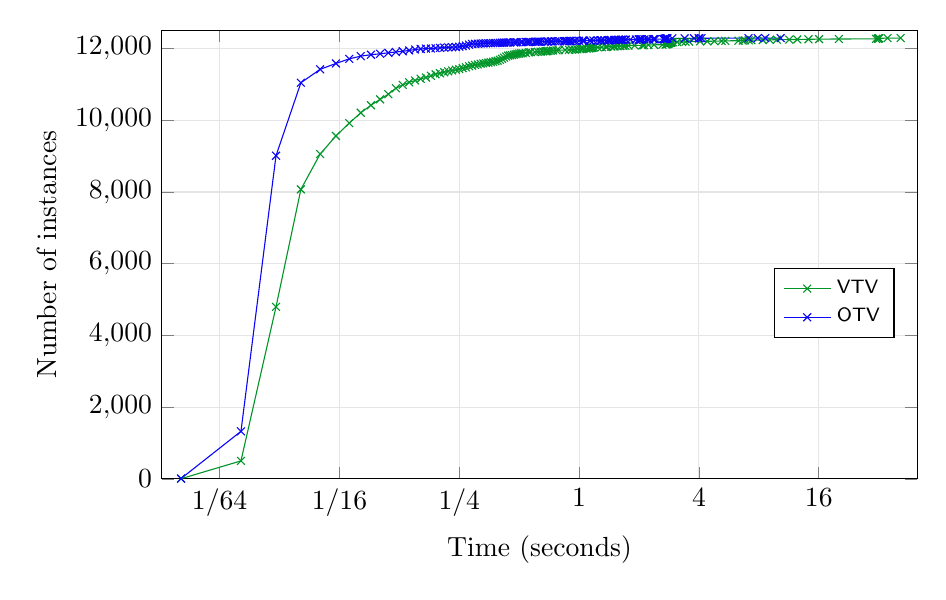
\begin{tikzpicture}[scale = 1.0]
    \begin{axis}
      [
        mark options={scale=1.0},
        grid=both, 
        grid style={black!10}, 
        xmode=log, 
        % ymode=log, 
        legend style={at={(0.97,0.47)}}, 
        legend cell align={left},
        x post scale=1.4, 
        y post scale=1.0, 
        xlabel=Time (seconds), 
        ylabel=Number of instances, 
        xtick={1000/64, 1000/16, 1000/4, 1000, 4000, 16000, 64000, 256000},
        xticklabels={1/64, 1/16, 1/4, 1, 4, 16, 64, 256},
        xmin=8,
        xmax=50000,
        ymin=0,
        ymax=12500, 
        scaled x ticks=false,
        scaled y ticks=false,
      ]

      \addplot[color=VTV, mark=x] coordinates { 
        (10, 5) (20, 502) (30, 4797) (40, 8072) (50, 9059) (60, 9562)
        (70, 9920) (80, 10208) (90, 10419) (100, 10582) (110, 10725) (120, 10892)
        (130, 10986) (140, 11057) (150, 11108) (160, 11156) (170, 11192) (180, 11239)
        (190, 11280) (200, 11310) (210, 11339) (220, 11365) (230, 11386) (240, 11409)
        (250, 11425) (260, 11451) (270, 11476) (280, 11504) (290, 11522) (300, 11543)
        (310, 11556) (320, 11574) (330, 11586) (340, 11594) (350, 11606) (360, 11620)
        (370, 11630) (380, 11646) (390, 11660) (400, 11685) (410, 11713) (420, 11744)
        (430, 11775) (440, 11801) (450, 11810) (460, 11816) (470, 11827) (480, 11840)
        (490, 11853) (500, 11860) (510, 11864) (520, 11869) (540, 11877) (560, 11891)
        (570, 11897) (600, 11901) (620, 11908) (640, 11912) (660, 11918) (680, 11923)
        (690, 11927) (700, 11931) (720, 11939) (740, 11943) (770, 11949) (790, 11953)
        (850, 11958) (890, 11962) (920, 11967) (950, 11971) (980, 11977) (1010, 11981)
        (1030, 11985) (1050, 11990) (1090, 11994) (1120, 12002) (1130, 12008) (1150, 12013)
        (1160, 12021) (1170, 12025) (1190, 12029) (1240, 12033) (1300, 12037) (1360, 12041)
        (1380, 12046) (1450, 12051) (1490, 12055) (1510, 12059) (1560, 12063) (1610, 12068)
        (1670, 12072) (1710, 12076) (1770, 12081) (1900, 12085) (2080, 12089) (2120, 12093)
        (2230, 12097) (2380, 12102) (2620, 12106) (2720, 12110) (2740, 12114) (2760, 12120)
        (2780, 12124) (2800, 12130) (2810, 12137) (2840, 12146) (2870, 12155) (2890, 12161)
        (2900, 12167) (2920, 12171) (2960, 12175) (3110, 12179) (3290, 12184) (3430, 12188)
        (3570, 12193) (4050, 12197) (4400, 12201) (4780, 12205) (5200, 12209) (5420, 12213)
        (6320, 12217) (6640, 12221) (6790, 12225) (7110, 12229) (7340, 12233) (8370, 12237)
        (9080, 12241) (9860, 12245) (11370, 12249) (12480, 12253) (14200, 12257) (16070, 12261)
        (20190, 12265) (31050, 12269) (31670, 12273) (31840, 12277) (31980, 12281) (32130, 12285)
        (35440, 12289) (41260, 12291)
      };

      \addplot[color=OTV, mark=x] coordinates { 
        (10, 10) (20, 1326) (30, 9011) (40, 11045) (50, 11419) (60, 11583)
        (70, 11711) (80, 11787) (90, 11827) (100, 11853) (110, 11879) (120, 11903)
        (130, 11922) (140, 11946) (150, 11973) (160, 11987) (170, 11998) (180, 12000)
        (190, 12010) (200, 12017) (210, 12025) (220, 12031) (230, 12036) (240, 12042)
        (250, 12049) (260, 12065) (270, 12082) (280, 12107) (290, 12127) (300, 12131)
        (310, 12134) (320, 12138) (330, 12142) (340, 12145) (350, 12147) (360, 12149)
        (370, 12150) (380, 12154) (390, 12157) (400, 12160) (410, 12161) (420, 12164)
        (430, 12165) (440, 12167) (450, 12168) (470, 12171) (480, 12173) (490, 12174)
        (510, 12177) (520, 12179) (540, 12180) (550, 12181) (560, 12182) (570, 12186)
        (600, 12187) (610, 12188) (620, 12189) (630, 12190) (640, 12192) (670, 12193)
        (690, 12194) (700, 12195) (720, 12197) (730, 12199) (760, 12200) (780, 12201)
        (800, 12202) (840, 12203) (850, 12205) (860, 12206) (870, 12207) (890, 12208)
        (900, 12209) (910, 12211) (940, 12213) (960, 12214) (1000, 12215) (1040, 12217)
        (1050, 12218) (1060, 12219) (1130, 12220) (1140, 12221) (1180, 12223) (1240, 12224)
        (1280, 12225) (1290, 12226) (1300, 12227) (1340, 12228) (1400, 12230) (1410, 12232)
        (1420, 12233) (1440, 12234) (1450, 12236) (1500, 12237) (1520, 12238) (1530, 12239)
        (1570, 12240) (1590, 12241) (1620, 12242) (1630, 12243) (1650, 12244) (1660, 12245)
        (1710, 12246) (1720, 12247) (1810, 12249) (1930, 12250) (2000, 12251) (2010, 12252)
        (2020, 12253) (2050, 12254) (2060, 12255) (2130, 12256) (2200, 12257) (2240, 12258)
        (2360, 12259) (2380, 12260) (2410, 12261) (2650, 12262) (2660, 12263) (2680, 12264)
        (2690, 12268) (2700, 12269) (2710, 12270) (2720, 12274) (2730, 12277) (2740, 12278)
        (2760, 12279) (2770, 12280) (2780, 12281) (2940, 12282) (3390, 12283) (3780, 12284)
        (3990, 12285) (4020, 12286) (4120, 12287) (7100, 12288) (7900, 12289) (8610, 12290)
        (10300, 12291)
      };
    
      \legend{
        \scriptsize \textsf{VTV}, 
        \scriptsize \textsf{OTV}
      }
    
    \end{axis}
  \end{tikzpicture}

  \caption{
    Verification times of VTV and OTV. The datapoints show the number of TESC proofs 
    that each verifier could check within the given time limit. The plots look more 
    ``jumpy'' toward the lower end due to the limited  time measurement resolution (10 ms) 
    of the unix \texttt{time} command.
  }
  \label{fig:time}
\end{figure}

VTV is slower than OTV as expected, but the difference is unlikely to be noticed 
in actual use since the absolute times for most proofs are very short, and the 
total times are dominated by a few outliers. 
VTV verified >97.4\% of proofs under 1 second, and >99.3\% under 5 seconds. 
Also, the median time for VTV is 40 ms, a mere 10 ms behind the OTV's 30 ms. 
But OTV's mean time (54.54 ms) is still much shorter than that of VTV (218.93 ms),
so users may prefer to use it for verifying one of the hard outliers or processing
a large batch of proofs at once.

The main drawback of VTV is its high memory consumption. Fig. \ref{fig:mem} shows
the peak memory usages of the two verifiers. For a large majority of proofs, 
memory usages of both verifiers are stable and stay within the 14-20 MB range,
but VTV's memory usage spikes earlier and higher than OTV. Due the limit of the system 
used, memory usage could only be measured up to 16 GB, but the actual peak for VTV 
would be higher if we included the 5 failed verifications. A separate test running 
VTV on an EC2 instance with 64 GB ram (\texttt{r5a.2xlarge}) still failed for 3 of 
the 5 problematic proofs, so the memory requirement for verifying all 12296 proofs 
with VTV is at least >64 GB. In contrast, OTV could verify all 
12296 proofs with less than 3.2 GB of memory.

\begin{figure}[tb]
  \centering
  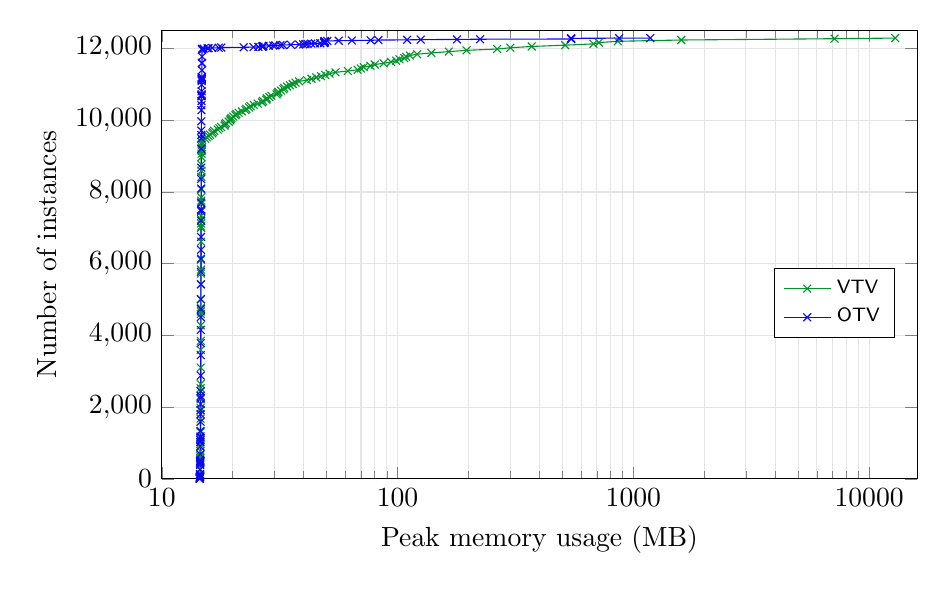
\begin{tikzpicture}[scale = 1.0]
    \begin{axis}
      [
        mark options={scale=1.0},
        grid=both, 
        grid style={black!10}, 
        xmode=log, 
        % ymode=log, 
        legend style={at={(0.97,0.47)}}, 
        legend cell align={left},
        x post scale=1.4, 
        y post scale=1.0, 
        xlabel=Peak memory usage (MB), 
        ylabel=Number of instances, 
        xtick={10000, 100000, 1000000, 10000000},
        xticklabels={10, 100, 1000, 10000},
        xmin=10000,
        xmax=16000000,
        ymin=0,
        ymax=12500, 
        scaled x ticks=false,
        scaled y ticks=false,
      ]

      \addplot[color=VTV, mark=x] coordinates { 
        (14472, 4) (14512, 55) (14536, 104) (14544, 277) (14548, 501) (14556, 573)
        (14564, 625) (14568, 673) (14572, 771) (14576, 894) (14584, 972) (14588, 1022)
        (14592, 1082) (14596, 1300) (14600, 1679) (14604, 1910) (14608, 1976) (14612, 2218)
        (14616, 2448) (14620, 2528) (14624, 2645) (14628, 3104) (14632, 3595) (14636, 3849)
        (14640, 4282) (14644, 4598) (14648, 4671) (14652, 4771) (14656, 5013) (14660, 5430)
        (14664, 5724) (14668, 5837) (14672, 6105) (14676, 6612) (14680, 6999) (14684, 7036)
        (14688, 7120) (14692, 7240) (14696, 7331) (14700, 7497) (14704, 7679) (14708, 7757)
        (14716, 7850) (14720, 8067) (14724, 8421) (14728, 8590) (14732, 8766) (14736, 8974)
        (14752, 9066) (14756, 9136) (14780, 9177) (14800, 9244) (14804, 9320) (14812, 9379)
        (14816, 9451) (15260, 9487) (15516, 9524) (15792, 9560) (16032, 9597) (16376, 9633)
        (16500, 9669) (16672, 9705) (17264, 9741) (17552, 9777) (17852, 9813) (18484, 9849)
        (18580, 9886) (18692, 9922) (19232, 9958) (19532, 9994) (19596, 10030) (19748, 10066)
        (20092, 10102) (20544, 10138) (20724, 10174) (21184, 10210) (21864, 10246) (22644, 10282)
        (22864, 10319) (23464, 10355) (23792, 10392) (24548, 10428) (25520, 10464) (26620, 10500)
        (26872, 10536) (27752, 10573) (27904, 10610) (28576, 10646) (29144, 10682) (30688, 10718)
        (30944, 10754) (31228, 10790) (32044, 10827) (32824, 10863) (33072, 10903) (33988, 10939)
        (34940, 10975) (35920, 11011) (36920, 11047) (38176, 11083) (41308, 11119) (43172, 11156)
        (45212, 11192) (47408, 11228) (49396, 11264) (51452, 11300) (54560, 11336) (61516, 11372)
        (67676, 11408) (69864, 11444) (71908, 11481) (76712, 11517) (80040, 11553) (87340, 11589)
        (93824, 11625) (98492, 11661) (101808, 11697) (106604, 11733) (108720, 11769) (112800, 11805)
        (121040, 11841) (139104, 11877) (164980, 11913) (196100, 11949) (264488, 11985) (300696, 12021)
        (370688, 12057) (513672, 12093) (677000, 12129) (714032, 12165) (859376, 12201) (1596720, 12237)
        (7129160, 12273) (12897180, 12291)
      };

      \addplot[color=OTV, mark=x] coordinates { 
        (14472, 6) (14496, 13) (14504, 28) (14508, 37) (14512, 48) (14524, 57)
        (14528, 68) (14532, 74) (14536, 107) (14540, 135) (14544, 253) (14548, 389)
        (14552, 424) (14556, 452) (14560, 474) (14564, 498) (14568, 535) (14572, 687)
        (14576, 912) (14580, 1030) (14584, 1076) (14588, 1145) (14592, 1183) (14596, 1336)
        (14600, 1594) (14604, 1804) (14608, 1914) (14612, 2089) (14616, 2254) (14620, 2314)
        (14624, 2441) (14628, 2881) (14632, 3452) (14636, 3785) (14640, 4155) (14644, 4511)
        (14648, 4733) (14652, 5010) (14656, 5422) (14660, 5776) (14664, 6142) (14668, 6386)
        (14672, 6746) (14676, 7199) (14680, 7461) (14684, 7512) (14688, 7706) (14692, 8095)
        (14696, 8361) (14700, 8679) (14704, 9205) (14708, 9491) (14712, 9591) (14716, 9712)
        (14720, 9969) (14724, 10281) (14728, 10418) (14732, 10533) (14736, 10666) (14740, 10681)
        (14744, 10696) (14748, 10722) (14752, 10807) (14756, 10991) (14760, 11093) (14764, 11124)
        (14768, 11146) (14776, 11154) (14780, 11176) (14784, 11195) (14792, 11206) (14800, 11396)
        (14804, 11590) (14808, 11600) (14812, 11773) (14816, 11966) (14820, 11979) (14832, 11985)
        (14836, 11991) (15072, 11997) (15620, 12003) (15796, 12009) (16364, 12015) (17436, 12021)
        (17880, 12027) (22252, 12033) (24480, 12039) (25684, 12045) (26656, 12051) (26752, 12057)
        (26880, 12063) (26956, 12069) (28436, 12075) (29684, 12081) (30296, 12087) (31860, 12093)
        (32656, 12099) (35272, 12105) (38244, 12111) (39820, 12117) (40676, 12123) (41460, 12129)
        (43032, 12135) (44632, 12141) (46996, 12147) (48872, 12154) (48900, 12161) (48924, 12168)
        (48956, 12175) (48964, 12181) (48996, 12187) (49032, 12193) (49088, 12199) (49116, 12205)
        (50372, 12211) (56284, 12217) (63976, 12223) (76892, 12229) (82960, 12235) (109728, 12241)
        (125312, 12247) (178576, 12253) (224040, 12259) (544396, 12265) (544488, 12271) (544532, 12277)
        (544688, 12283) (870444, 12289) (1179916, 12291)
      };
    
      \legend{
        \scriptsize \textsf{VTV}, 
        \scriptsize \textsf{OTV}
      }
    
    \end{axis}
  \end{tikzpicture}

  \caption{
    Peak memory usages of VTV and OTV. The datapoints show the number of TESC proofs 
    that each verifier could check within the given peak memory usage. 
  }
  \label{fig:mem}
\end{figure}

\section{Conclusion}  \label{sec:conclusion}

The robust test results show that VTV can serve as a fallback option when extra rigour 
is required in verification, thereby increasing our confidence in the correctness of TESC proofs. 
It can also help the design of other TESC verifiers by providing a reference implementation 
that is guaranteed to be correct. On a more general note, VTV is an example of a first-order logic 
formalization that strikes a practical balance between ease of proofs and efficient computation 
while avoiding some common pitfalls like non-termination and complex arity checking. 
Therefore, it can provide a useful starting point for other verified programming projects 
that use first-order logic.

There are two main ways in which VTV could be further improved. Curbing its 
memory usage would be the most important prerequisite for making it the 
default verifier in T3P. This may require porting VTV to a verified programming
language with finer low-level control over memory usage. 

VTV could also benefit from a more reliable TPTP parser. A formally verified 
parser would be ideal, but the complexity of TPTP's syntax makes it difficult  
to even \textit{specify} the correctness of a parser, let alone prove it. 
A more realistic approach would be imitating the technique used by verified 
LRAT checkers \cite{heule2017efficient}, making VTV print the parsed problem 
and textually comparing its output with the original problem.



\section*{Acknowledgements}  \label{sec:ack}

This work has been partially supported by AFOSR grant FA9550-18-1-0120.

Thanks to Jeremy Avigad for a careful proofreading of drafts and advice for improvements.



\bibliographystyle{plain}

\bibliography{references}



\appendix  

\section{Formula analysis functions} \label{apdx:faf}

\begin{centering}
    \begin{tabular}{|c|cc|}
    \hline
    A & 
    {
      $\begin{aligned}
        A(0, \lnot (\phi \lor \psi)) =&\ \lnot \phi\\ 
        A(0, \phi \land \psi) =&\ \phi\\ 
        A(0, \lnot (\phi \to \psi)) =&\ \phi\\ 
        A(0, \phi \liff \psi) =&\ \phi \limp \psi
      \end{aligned}$
    } &  
    {
      $\begin{aligned}
        A(1, \lnot (\phi \lor \psi)) =&\ \lnot \psi\\
        A(1, \phi \land \psi) =&\  \psi\\
        A(1, \lnot (\phi \to \psi)) =&\  \lnot \psi\\
        A(1, \phi \liff \psi) =&\  \psi \limp \phi
      \end{aligned}$
    } 
    \\ \hline
    B &
    {
      $\begin{aligned}
        B(0, \phi \lor \psi) =&\  \phi\\ 
        B(0, \lnot (\phi \land \psi)) =&\  \lnot \phi\\ 
        B(0, \phi \to \psi) =&\  \lnot \phi\\ 
        B(0, \lnot (\phi \liff \psi)) =&\  \lnot \phi \limp \psi
      \end{aligned}$
    } &  
    {
      $\begin{aligned}
        B(1, \phi \lor \psi) =&\  \psi\\
        B(1, \lnot (\phi \land \psi)) =&\  \lnot \psi\\
        B(1, \phi \to \psi) =&\  \psi\\
        B(1, \lnot (\phi \liff \psi)) =&\  \lnot \psi \limp \phi
      \end{aligned}$
    } 
    \\ \hline
    C & 
    $C(t, \forall \phi) = \phi [0 \mapsto t]$ &
    $C(t, \lnot \exists \phi) = \lnot \phi [0 \mapsto t]$
     \\ \hline
    D & 
    $D(k, \exists \phi) = \phi [0 \mapsto \idf{k}]$) &
    $D(k, \lnot \forall \phi) = \lnot \phi [0 \mapsto \idf{k}]$ 
    \\ \hline
    N & \multicolumn{2}{c|}{$N(\lnot \lnot \phi) = \phi$} 
    \\ \hline
  \end{tabular}
  
\end{centering}

\vspace{5mm}

    The Formula analysis functions used by analytic rules. For any argument not explicitly 
    defined above, the functions all return $\top$. E.g., $A(0, \phi \lor \psi) = \top$.
    $\phi[k \mapsto t]$ denotes the result of replacing all variables in $\phi$ bound 
    to the $k$th quantifier with term $t$. For the exact definition of substitutions 
    using De Bruijn indices, see Appendix \ref{apdx:subst}.


\end{document}

















